\documentclass[lualatex,book,paper=a4paper,jafontsize=11.5pt,jafontscale=1.05,openany]{jlreq}

%フォント:
\usepackage{luatexja-fontspec}
\usepackage{hack-fonts}

%表紙用:
\usepackage{hack-cover}

% リンク
\usepackage[hidelinks]{hyperref}

% 画像
\usepackage{graphicx}

%表
\usepackage{hhline}
% \sisetup{output-decimal-marker = {.}} % 

% 単位 
\usepackage{siunitx}



\title{ハッカソン}
\subtitle{～計画書と設計書～}
\team{チーム40}
\author{
	24G1021 : 宇井 祐真\\
        24G1026 : 梅野 大誠\\
	24G1136 : 山口 侑希 \\
        25G1020 : 薄井 悠希\\
        25G1041 : 菊池 侑人\\
        25G1059 : 佐藤 涼菜  
        }
\date{\today}
\version{x.x}

%%%%%%%%%%%%%%%%%%%%%%%%%%%%%%%%%%%%%%%%%%%%%%%%
\begin{document}
\maketitle

\setcounter{tocdepth}{2}
\tableofcontents 
\thispagestyle{empty}


% %%%%%%%%%%%%%%%%%%%%%%%%
% %%%%%%%%%%%%%%%%%%%%%%%%
% %%%%%%%%%%%%%%%%%%%%%%%%
% \chapter{プロジェクトの計画書} \label{chap:project-plan}\setcounter{page}{1}


% %%%%%%%%%%%%%%%%%%%%%%%%
% \section{プロジェクトの概要}
% %%%%%%%%%%%%%%%%%%%%%%%%
% \subsection{プロジェクトの題目}

% %%%%%%%%%%%%%%%%%%%%%%%%
% \subsection{プロジェクトの目的}
% プロジェクトの目的と最終的なゴール，解決すべき課題を記述する．

% %%%%%%%%%%%%%%%%%%%%%%%%
% \subsection{既存の技術とプロジェクトの独自性}

% %%%%%%%%%%%%%%%%%%%%%%%%
% %%%%%%%%%%%%%%%%%%%%%%%%
% \section{スコープ・マネジメント}
% %%%%%%%%%%%%%%%%%%%%%%%%
% \subsection{成果物}

% %%%%%%%%%%%%%%%%%%%%%%%%
% \subsection{プロジェクトの対象範囲と非対象範囲}

% %%%%%%%%%%%%%%%%%%%%%%%%
% \subsection{機能分解構造FBS}

% %%%%%%%%%%%%%%%%%%%%%%%%
% \subsection{製品分解構造PBS}

% %%%%%%%%%%%%%%%%%%%%%%%%
% \subsection{FBSとPBSの対応関係}


% %%%%%%%%%%%%%%%%%%%%%%%%
% %%%%%%%%%%%%%%%%%%%%%%%%
% \section{作業計画}
% %%%%%%%%%%%%%%%%%%%%%%%%
% \subsection{作業分解構造WBSと管理番号}

% %%%%%%%%%%%%%%%%%%%%%%%%
% \subsection{アローダイアグラムとクリティカルパス}

% %%%%%%%%%%%%%%%%%%%%%%%%
% \subsection{役割分担}

% %%%%%%%%%%%%%%%%%%%%%%%%
% \subsection{ガントチャート}


% %%%%%%%%%%%%%%%%%%%%%%%%
% %%%%%%%%%%%%%%%%%%%%%%%%
% \section{検証と妥当性確認: V\&V計画}
% %%%%%%%%%%%%%%%%%%%%%%%%
% \subsection{プロジェクトの成果物に対する有効指標MOE}

% %%%%%%%%%%%%%%%%%%%%%%%%
% \subsection{有効指標MOEに対応する性能指標MOP}

% %%%%%%%%%%%%%%%%%%%%%%%%
% \subsection{システムテストで評価する性能指標MOP}

% %%%%%%%%%%%%%%%%%%%%%%%%
% \subsection{結合テストで評価する性能指標MOP}

% %%%%%%%%%%%%%%%%%%%%%%%%
% \subsection{単体テストで評価する性能指標MOP}

% %%%%%%%%%%%%%%%%%%%%%%%%
% \subsection{プロジェクト中に監視する技術性能指標TPM}

% %%%%%%%%%%%%%%%%%%%%%%%%
% \subsection{プロジェクト中に監視する指標TPM}


% %%%%%%%%%%%%%%%%%%%%%%%%
% %%%%%%%%%%%%%%%%%%%%%%%%
% \section{資源・調達管理}


% %%%%%%%%%%%%%%%%%%%%%%%%
% %%%%%%%%%%%%%%%%%%%%%%%%
% \section{リスク管理}


%%%%%%%%%%%%%%%%%%%%%%%%
%%%%%%%%%%%%%%%%%%%%%%%%
%%%%%%%%%%%%%%%%%%%%%%%%
\chapter{システムの基本設計}

% 設計書は作成する成果物によって変化します．
% 適宜修正して利用してください．


%%%%%%%%%%%%%%%%%%%%%%%%
\section{機能一覧}
% 機能分解構造FBSの要素の説明
%指揮デバイスの機能と楽器鳴らすデバイスに付随するセンサ
本節では指揮デバイスと楽器デバイスの機能について説明する．
まず指揮デバイスについて説明する．
指揮デバイスとは演奏全体を統括するデバイスであり，主に以下の三つの機能を有する．
第一の機能は，演奏開始トリガーの送信である．ユーザが指揮デバイスを上下に振ると，内蔵の加速度センサが振り動作に伴う加速度を検知する．そして，
この値が設定した閾値を超過した瞬間に，観覧車デバイスと楽器デバイスへ演奏開始の情報を送信する．
第二の機能は，楽曲のBPM変更である．ユーザが操作をすると新しい設定BPM情報が観覧車デバイスへ送信される．これにより，観覧車のモータ回転速度がこの値に
追従して変化する．そして，その回転に伴うLEDの通過光を介して各楽器デバイスに情報が伝達され，リアルタイムに楽曲のBPMが変更および同期される．
第三に，楽曲の音量変更である．ユーザが操作をすると音量情報が各楽器デバイスへブロードキャスト送信されることで楽曲の音量がリアルタイムに変更される．\par

次に，楽器デバイスについて説明する．
楽器デバイスは観覧車デバイスの回転状態を基準として，自律的に演奏を行うデバイスであり，主に以下の四つの機能を有する．
第一の機能は，演奏開始の検知である．光センサが観覧車デバイスのLED光を初回に検知した際，楽曲の再生を開始する．
第二の機能は，楽曲のBPMリアルタイム同期である．演奏開始後もLED光の通過間隔を常時計測し，その間隔から現在のBPMを逐次算出する．
第三の機能は，楽器の音色再生である．ArduinoとUSBケーブルで接続されたPC上のProcessingを用いることで，各楽器の音色を出力し，演奏を再現する．
第四に，楽曲の音量リアルタイム反映である．指揮デバイスから受け取った音量情報をProcessingへ送信し，再生中の出力音量へ反映する．



%%%%%%%%%%%%%%%%%%%%%%%%
\section{システム構成図}
% ハードウェア，ソフトウェアなどの構成図を記載する．
本節では指揮デバイスのシステム構成および楽器デバイスの受光機構のシステム構成について説明する．

指揮デバイスのシステム構成図を図\ref{fig:sys_siki}に示す．本デバイスは内蔵の加速度センサによりデバイスの振り動作を検知すると，各楽器デバイスとの中継を担う観覧車デバイスへ演奏開始情報を無線送信し，
演奏を開始させる．また，ユーザによる操作により楽曲のBPMを自由に変更できる．
% また，ユーザによる操作により楽曲のBPMを変更することが可能であり，その情報は観覧車デバイスへ無線送信され，観覧車デバイスの回転を介して各楽器デバイスへと伝達される．



\begin{figure}[htbp] % h:ここ, t:上, b:下, p:独立ページ
        \centering % 中央揃え
        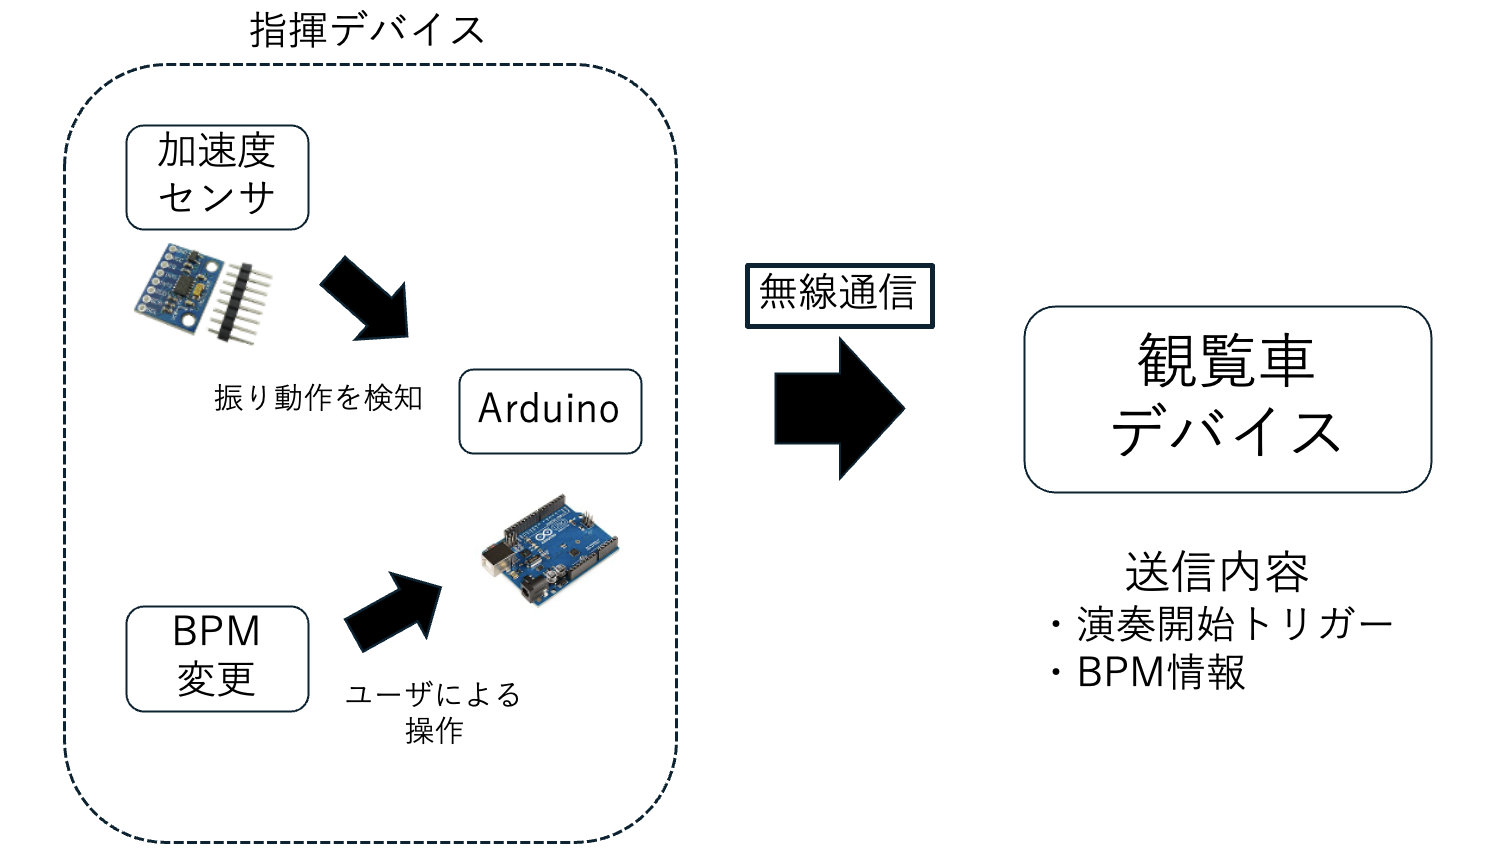
\includegraphics[width=0.8\columnwidth]{siki_sys2.png} % 横幅を列幅の80%に指定
        \caption{指揮デバイスのシステム構成図} % 図の説明
        \label{fig:sys_siki} % 本文中で参照するためのラベル
\end{figure}



次に，楽器デバイス受光機構のシステム構成図を図\ref{fig:jusin_sys}に示す．
本機構は，回転している観覧車デバイスのLED光を検知することで楽器の同期を維持する．
あらかじめ設定した位置に各楽器デバイスを設置し，観覧車デバイスのLEDが通過した瞬間に光センサがこの光を検知することで，
演奏の同期およびBPMの変更が行われる．また，初回に観覧車デバイスからの光を受光した際は，楽曲の再生を開始する．
% また，観覧車デバイスの中心にある中継機Arduinoからの無線通信により音量情報を受信することで楽曲の音量が変更できる．

\begin{figure}[htbp] % h:ここ, t:上, b:下, p:独立ページ
        \centering % 中央揃え
        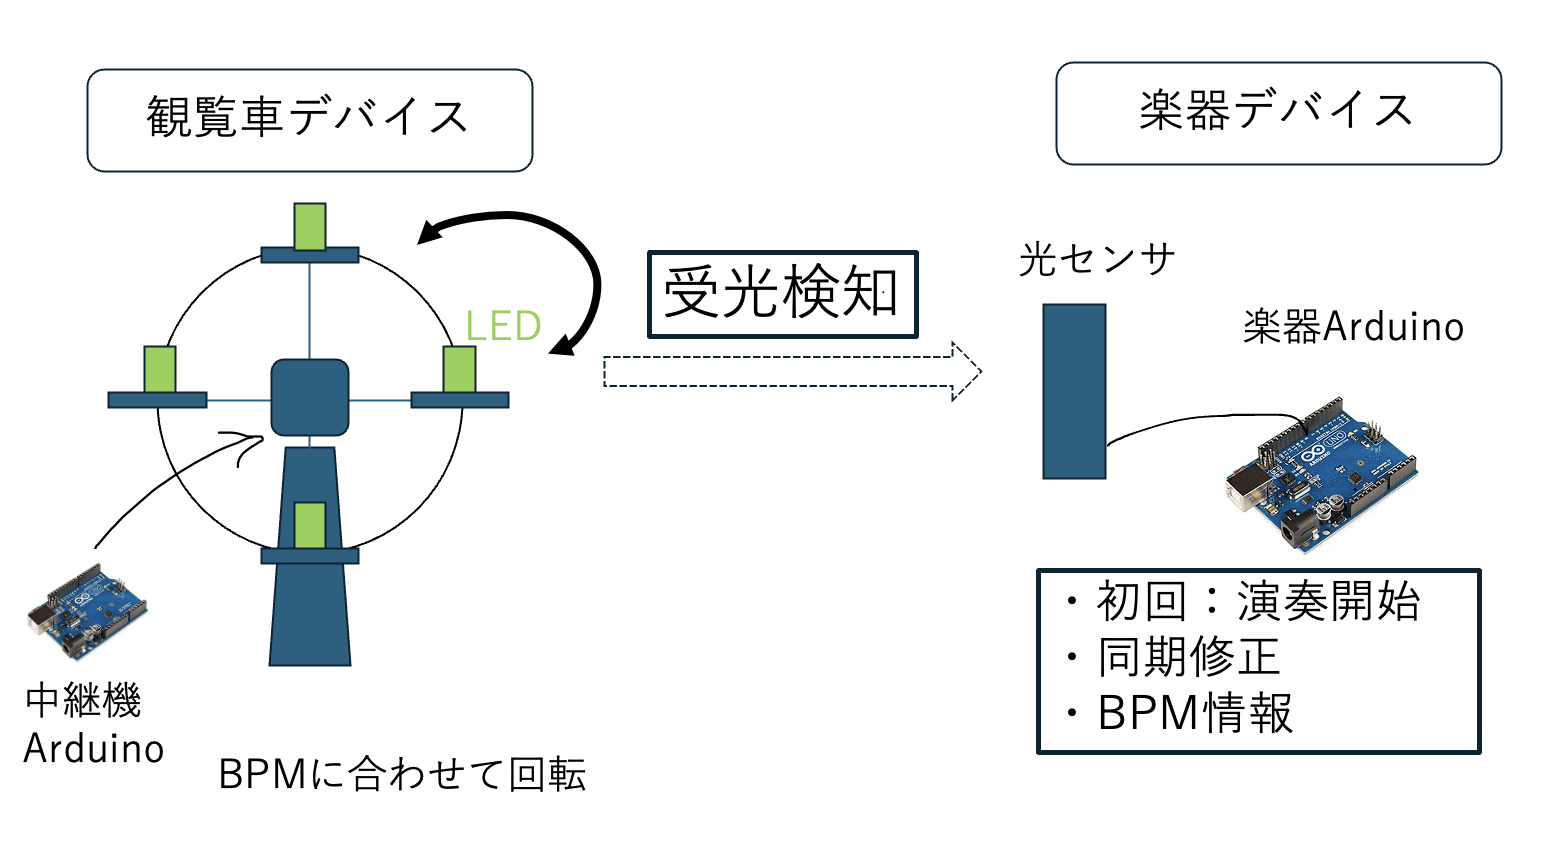
\includegraphics[width=0.8\columnwidth]{jusin_sys2.png} % 横幅を列幅の80%に指定
        \caption{楽器デバイスの受光機構のシステム構成図} % 図の説明
        \label{fig:jusin_sys} % 本文中で参照するためのラベル
\end{figure}


\newpage

%%%%%%%%%%%%%%%%%%%%%%%%
\section{操作インターフェース設計}
% 画面やスイッチなどのインターフェースの設計図を記載する
本節では指揮デバイスの設計および指揮デバイスの演奏開始トリガー送信機構とBPM変更機構の操作インターフェース設計について説明する．なお，
楽器デバイスのの受光部はユーザの直接操作が存在しないため，操作インターフェース設計の対象外とする．

指揮デバイスの設計について図\ref{fig:inta_siki_mitame}に示す．
本デバイスは，実際の指揮棒のようにユーザが片手で振って操作できるよう，細長い筒状の外装を採用する．
また，内部のブレッドボードに加速度センサや可変抵抗器を設置し，ユーザが操作しやすいようスライダー部分は外部へ露出させる
構造とする．さらに，指揮デバイスの先端部に加速度センサを，後端部に外部電源を設置することで，操作時の重心を安定させユーザビリティを向上させる．


\begin{figure}[htbp] % h:ここ, t:上, b:下, p:独立ページ
        \centering % 中央揃え
        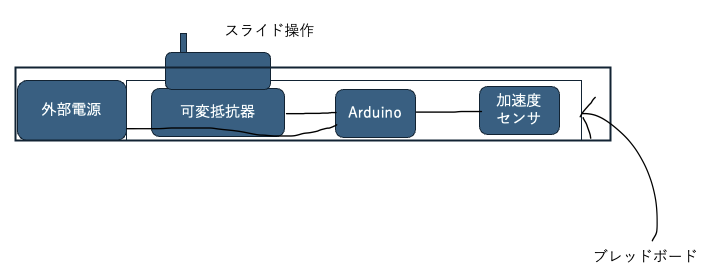
\includegraphics[width=0.8\columnwidth]{siki_mitame.png} % 横幅を列幅の80%に指定
        \caption{指揮デバイス設計} % 図の説明
        \label{fig:inta_siki_mitame} % 本文中で参照するためのラベル
\end{figure}



次に，指揮デバイスの演奏開始トリガー送信機構の設計について図\ref{fig:inta_kaisi}に示す．
本機構は，ユーザが指揮デバイスを上下に振ることで演奏を開始させる．指揮デバイスに内蔵の加速度センサが振り動作の加速度を検知し，その値が
閾値を超過すると，観覧車デバイスへ演奏開始情報が無線送信され回転を開始する．また，楽器デバイスへ演奏を開始するための信号を送信する．

% そして，観覧車デバイスが回転を開始し，そのLED光を楽器デバイスの受光部が
% 検知することで，楽曲が再生される仕様である．

\begin{figure}[htbp] % h:ここ, t:上, b:下, p:独立ページ
        \centering % 中央揃え
        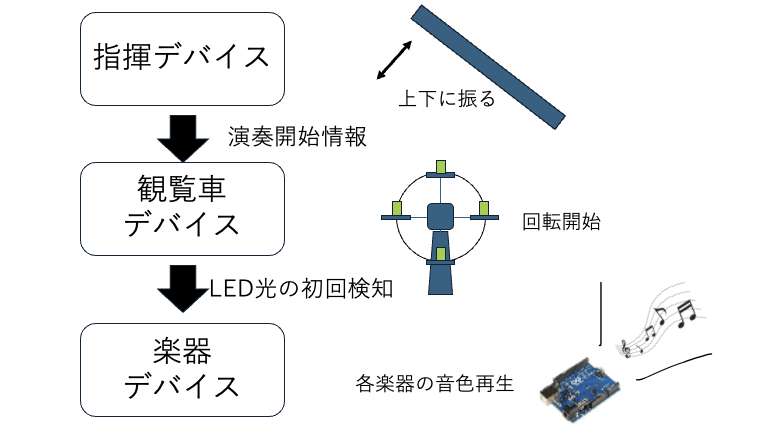
\includegraphics[width=0.8\columnwidth]{kaisi_inta.png} % 横幅を列幅の80%に指定
        \caption{演奏開始トリガー送信機構設計} % 図の説明
        \label{fig:inta_kaisi} % 本文中で参照するためのラベル
\end{figure}



\newpage
最後に，指揮デバイスのBPM変更機構の設計について図\ref{fig:inta_siki}に示す．本機構は，ユーザがスライド式可変抵抗器を操作することで楽曲のBPMが自由に変更できる．
ユーザがスライド式可変抵抗器をスライドすると，新しい設定BPM情報が観覧車デバイスへ無線送信される．これにより，観覧車デバイスの回転速度がこの値に追従して変化し，その
回転を介して各楽器デバイスへ情報が伝達されることで，楽器のBPMが変更される．この一連の処理によって観覧車デバイスの回転速度と楽曲のBPMが常に同期される仕様である．

% また音量変更は，BPMと同様にユーザがスライド式可変抵抗器をスライドすると各楽器用Arduinoに情報が送信され変更される．


\begin{figure}[htbp] % h:ここ, t:上, b:下, p:独立ページ
        \centering % 中央揃え
        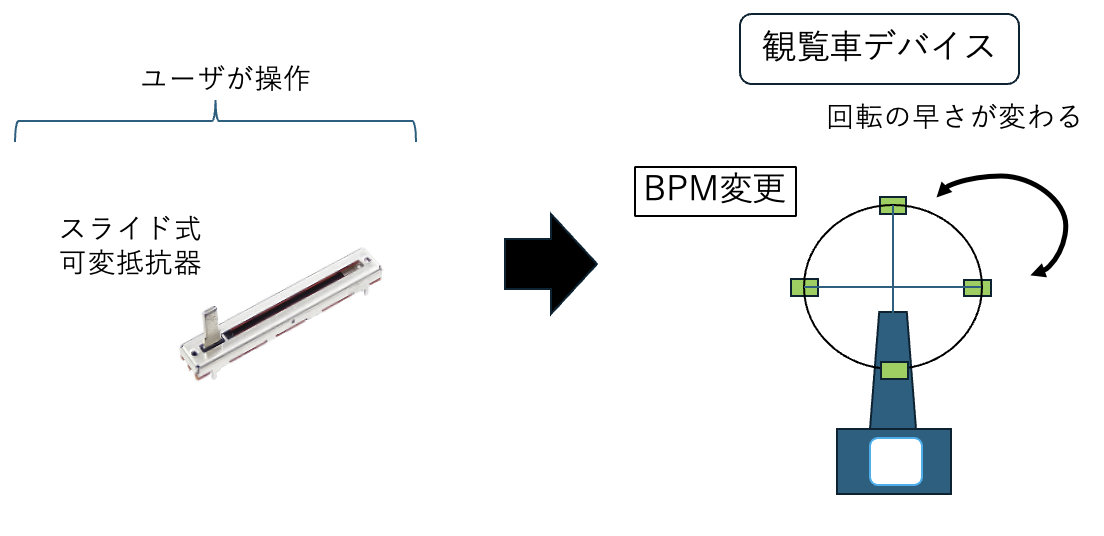
\includegraphics[width=0.8\columnwidth]{siki_inta2.png} % 横幅を列幅の80%に指定
        \caption{BPM変更機構設計} % 図の説明
        \label{fig:inta_siki} % 本文中で参照するためのラベル
\end{figure}










%%%%%%%%%%%%%%%%%%%%%%%%
\newpage
\section{シーケンス図}
本節では指揮デバイスおよび楽器デバイス受光機構における状態遷移について説明する．

まず，指揮デバイスのシーケンス図を図\ref{fig:jou_siki}に示す．
ユーザが指揮デバイスを上下に振ると加速度センサが動作を検知しArduinoに送信される．この時，値が閾値を超過した場合，
観覧車デバイスと無線通信が開始し初期BPMおよび音量情報が送信され演奏が開始する．また，演奏中はユーザによるスライド操作によって
楽曲のBPMの値を自由に変更できる．

\begin{figure}[htbp] % h:ここ, t:上, b:下, p:独立ページ
        \centering % 中央揃え
        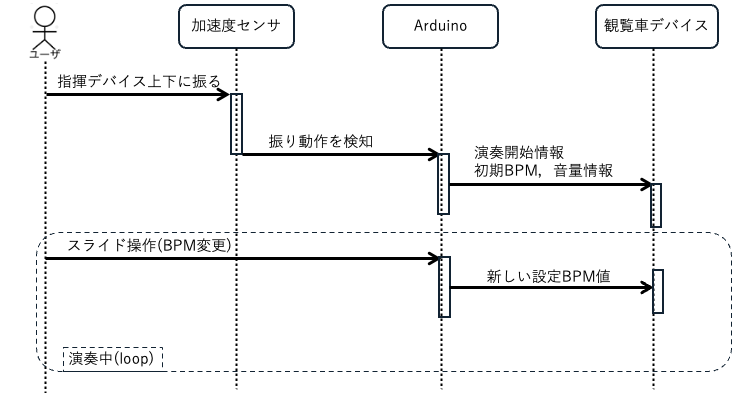
\includegraphics[width=0.8\columnwidth]{siki_jou4.png} % 横幅を列幅の80%に指定
        \caption{指揮デバイスのシーケンス図} % 図の説明
        \label{fig:jou_siki} % 本文中で参照するためのラベル
\end{figure}



次に，楽器デバイスの受光機構のシーケンス図を図\ref{fig:jou_jusin}に示す．
観覧車デバイスのLED光が初回に通過した際，光センサが楽器デバイス内のArduinoへデジタル信号を送信し，PCから楽器の音色が再生される．
演奏中は観覧車デバイスのLED光が楽器デバイスの受光部を通過するごとに光センサがArduinoへデジタル信号を送信する．この通過間隔から
BPMを算出することで，最新のBPM値をPCへ送信する．

\begin{figure}[htbp] % h:ここ, t:上, b:下, p:独立ページ
        \centering % 中央揃え
        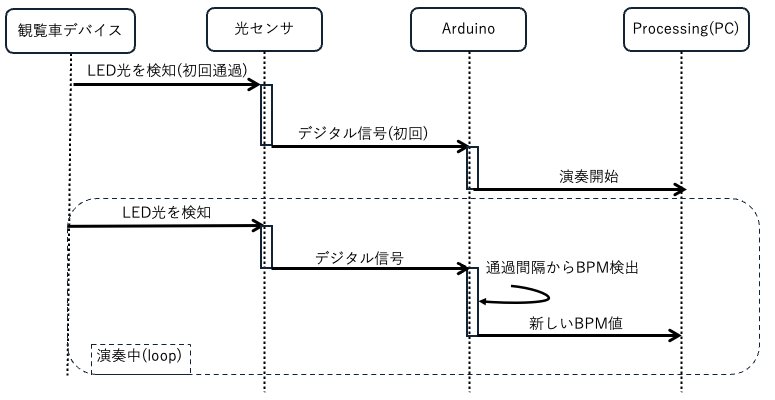
\includegraphics[width=0.8\columnwidth]{jusin_jou4.png} % 横幅を列幅の80%に指定
        \caption{楽器デバイスの受光機構のシーケンス図} % 図の説明
        \label{fig:jou_jusin} % 本文中で参照するためのラベル
\end{figure}



%%%%%%%%%%%%%%%%%%%%%%%%
%%%%%%%%%%%%%%%%%%%%%%%%
%%%%%%%%%%%%%%%%%%%%%%%%
\chapter{システムの詳細設計}

% 設計書は作成する成果物によって変化します．
% 適宜修正して利用してください．


%%%%%%%%%%%%%%%%%%%%%%%%
\section{部品一覧}
% 製品分解構造PBSの要素の説明

本節では，指揮デバイスおよび楽器デバイスの受光部を構成する部品について説明する．

指揮デバイスを構成する部品について表\ref{table:siki}に示す．
デジタル3軸加速度センサは指揮デバイスの動きの検知に使用し，スライド式可変抵抗器は
BPM変更に使用される．また，指揮デバイスの電力供給源として$\SI{9}{V}$の乾電池を外部電源として使用する．

\begin{table}[h]
  \centering
  \caption{使用機器}
  \label{table:siki}
  \begin{tabular}{c|c|c}
  
  \hline
  部品名 & 数量 & 仕様 \\\hline\hline
  Arduino UNO R4 & 1 & マイコン\\\hline
  スライド式可変抵抗器 & 1 & $\SI{10}{kΩ}$\\\hline
  デジタル3軸加速度センサ & 1 & GY-291\\\hline
  外部電源 & 1 & $\SI{9}{V}$\\\hline

  \end{tabular}
\end{table}

次に，楽器デバイスが受光するための部品について表\ref{table:ota}に示す．
光センサモジュールとしてLM393搭載フォトダイオードモジュールを使用する．
本モジュールはコンパレータ(LM393)を内蔵しており，受光量が設定した閾値を超えた瞬間にデジタル信号を出力する．
この出力をArduinoのDピンへ接続することで，観覧車デバイスのLEDの通過を検知する．また，今回はドラム，ピアノ，チェロ，フルートの4種類の
楽器の音色を再現するためにそれぞれにArduinoを使用するため，光センサおよびブレッドボードも4台用意する．




\begin{table}[h]
        \centering
        \caption{使用機器}
        \label{table:ota}
        \begin{tabular}{c|c|c}
        
        \hline
        部品名 & 数量 & 仕様 \\\hline\hline
        Arduino UNO R4 & 4 & マイコン\\\hline
        光センサ & 4 & uxcell フォトダイオードモジュール\\\hline
        ブレッドボード & 4 & 16401020E\\\hline
      
        \end{tabular}
\end{table}

%%%%%%%%%%%%%%%%%%%%%%%%
%%%%%%%%%%%%%%%%%%%%%%%%
\section{ハードウェア設計}

本節では指揮デバイスおよび楽器デバイスの受光部のハードウェア設計について説明する．

まず，指揮デバイスの回路図を図\ref{fig:kairo_siki}に示す．
電源仕様は，$\SI{9}{V}$乾電池をArduinoのVINピンに入力することで，Arduino内蔵の電圧レギュレータが$\SI{5}{V}$および$\SI{3.3}{V}$に降圧し，
各モジュールへ安定した電力を供給する．
また，加速度センサはI2C通信によりArduinoと接続するためCSピンはArduinoの$\SI{3.3}{V}$に接続している．SDOをGNDに接続することで，I2Cアドレスを0x53に固定する．
SDAピンはデータをやり取りするため，SCLピンは通信のタイミングをあわせるクロック信号を送るためにそれぞれArduinoのA4，A5ピンに接続している．
また，指揮デバイスの振り動作による加速度が内部設定の閾値を超過した場合，INT1ピンからD2ピンへ割り込み信号を出力しモータ制御用Arduinoとの通信が開始される．


\begin{figure}[htbp] % h:ここ, t:上, b:下, p:独立ページ
        \centering % 中央揃え
        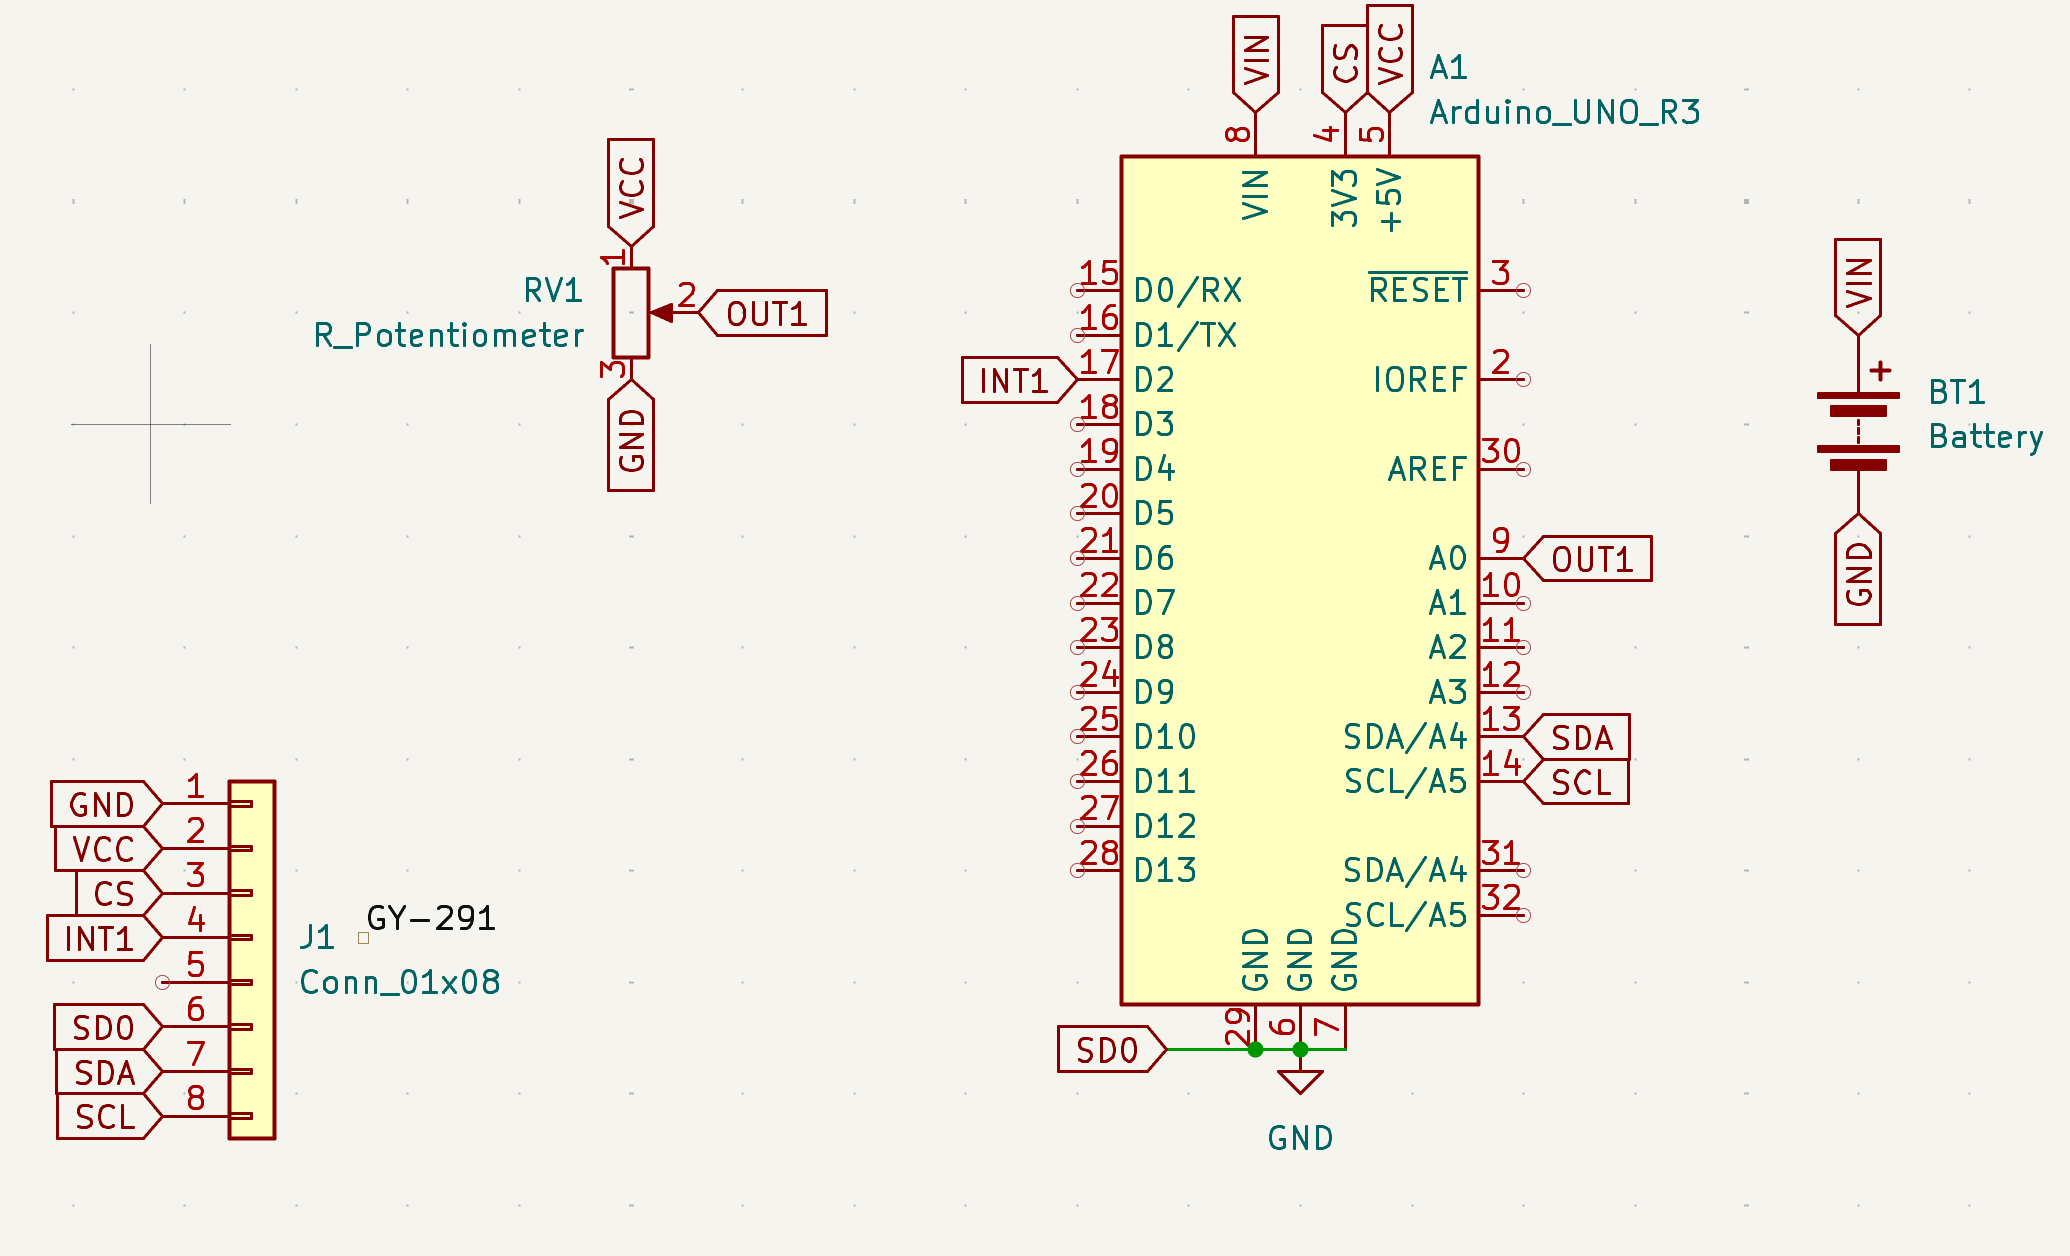
\includegraphics[width=0.8\columnwidth]{kairo_siki2.png} % 横幅を列幅の80%に指定
        \caption{指揮デバイスの回路図} % 図の説明
        \label{fig:kairo_siki} % 本文中で参照するためのラベル
\end{figure}

\newpage

次に，楽器デバイスの受光部の回路図を図\ref{fig:kairo_hikari}に示す．
電源仕様は，PCとのUSB接続から電力を供給する．光センサはArduinoの$\SI{5}{V}$ピンから給電されるため，外部電源は不要である．
また，光センサが光を受光した瞬間にD2へデジタル信号を出力し，ArduinoのD2ピンで処理されることで光を検知する仕様である．
A0ピンへのアナログ出力はデバッグ時に光量の変化を確認するために使用する．

\begin{figure}[htbp] % h:ここ, t:上, b:下, p:独立ページ
        \centering % 中央揃え
        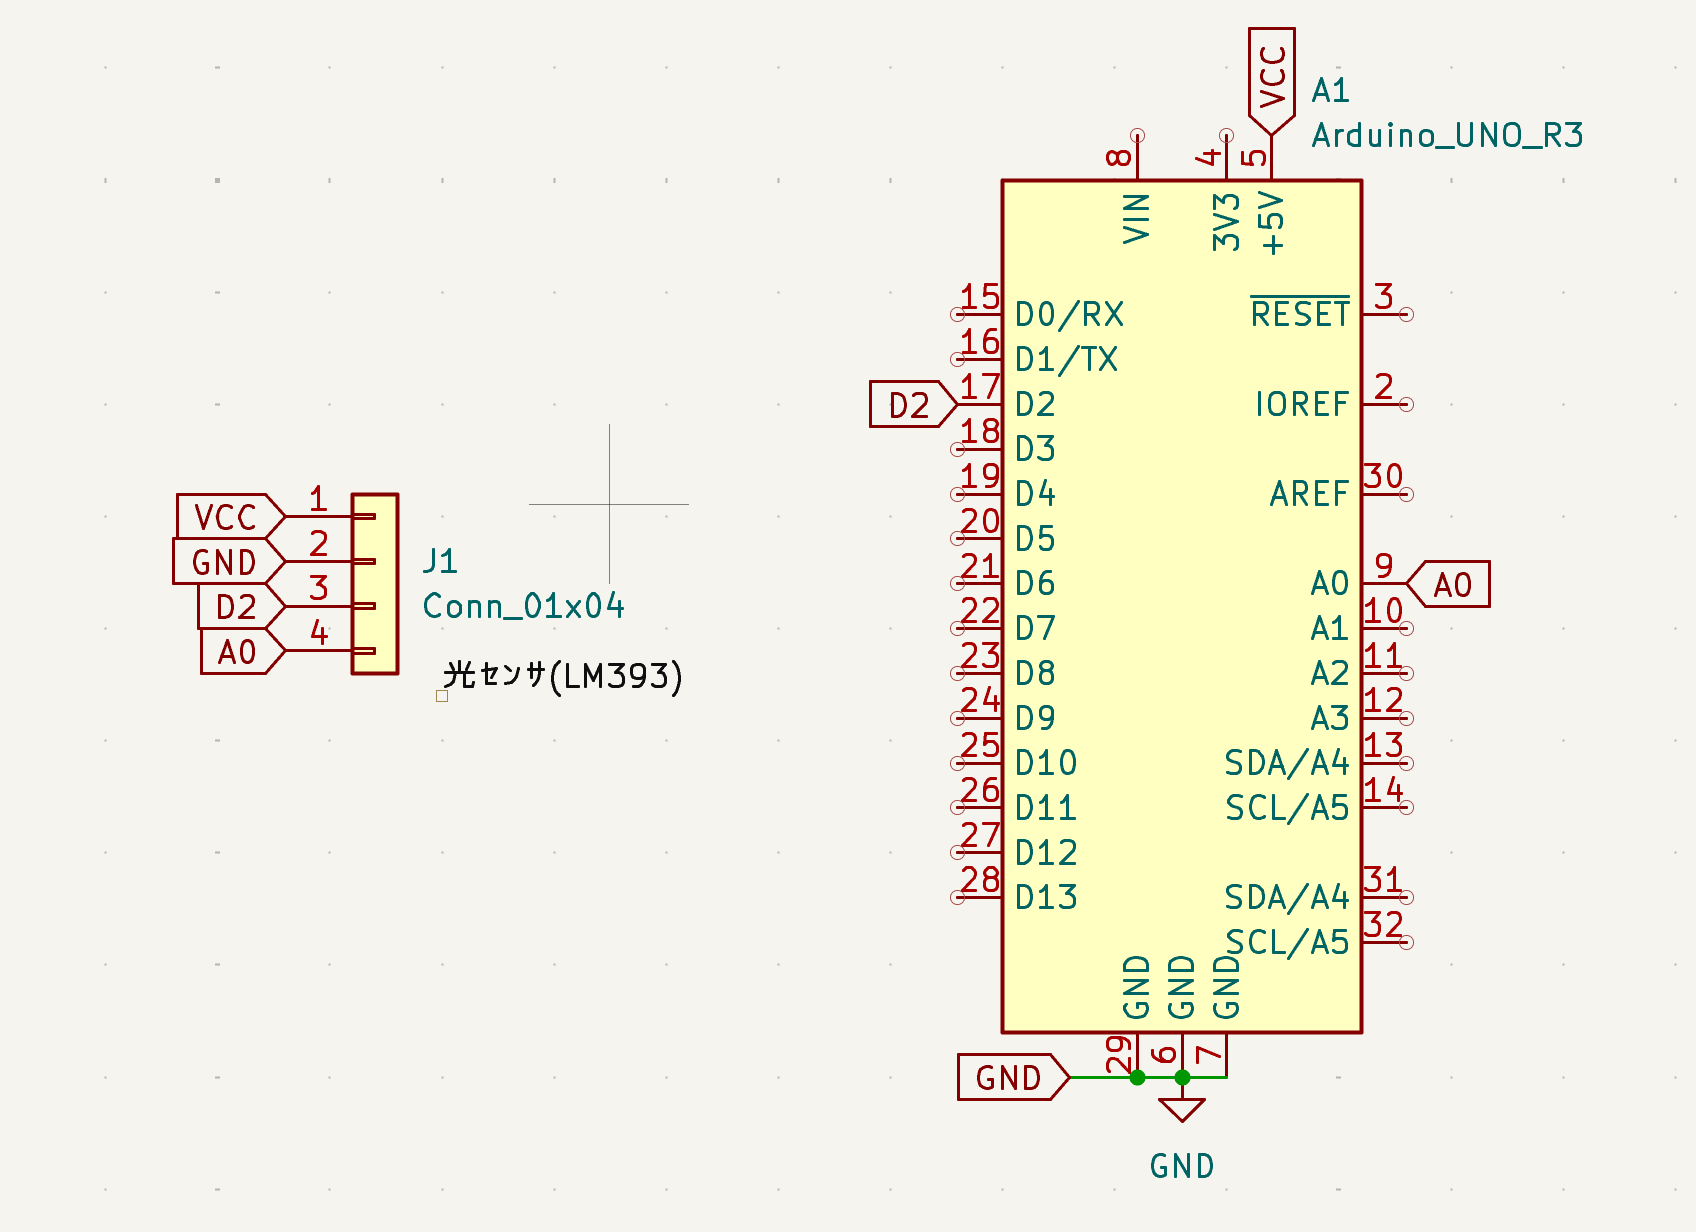
\includegraphics[width=0.8\columnwidth]{kairo_hikari.png} % 横幅を列幅の80%に指定
        \caption{楽器デバイスの受光部の回路図} % 図の説明
        \label{fig:kairo_hikari} % 本文中で参照するためのラベル
\end{figure}


%%%%%%%%%%%%%%%%%%%%%%%%
%%%%%%%%%%%%%%%%%%%%%%%%
% \section{ソフトウェア設計}

% %%%%%%%%%%%%%%%%%%%%%%%%
% \subsection{ファイル構成}

% %%%%%%%%%%%%%%%%%%%%%%%%
% \subsection{オブジェクト設計(クラス図)}

% %%%%%%%%%%%%%%%%%%%%%%%%
% \subsection{関数設計}


%%%%%%%%%%%%%%%%%%%%%%%%
%%%%%%%%%%%%%%%%%%%%%%%%
% \section{処理フローの設計}


%%%%%%%%%%%%%%%%%%%%%%%%
%%%%%%%%%%%%%%%%%%%%%%%%
\newpage
\section{テストの設計}
% どのようにテストを行うのか，例えば，テストデータの設計などを記述．
% 不快に感じる程度の遅延がないか　ー＞　50ms以内
% 音が再現できているか　　　　　　ー＞　アンケートをとる(MOS評価).中央値，最頻値を使って4.0以上目指す．
% BPMの回転速度がずれていないか   ー＞　回転速度とBPMのズレがn以内
% エンターテイメント性はあるか　　ー＞　CSATで75%以上の範囲

本節では指揮デバイスおよび楽器デバイスの受光部のテスト設計について説明する．
開発したシステムが設計どおりの機能を持つか評価するために，今回は通信遅延を$\SI{50}{ms}$以内に収めることを指標とする．
この値は，先行研究から人間が演奏遅延により不快感を抱かない範囲であることが示されている\cite{ref:tien}．したがって，
全体の通信遅延を$\SI{50}{ms}$以内に収めることを目的とする．

また，指揮デバイスが振り動作を検知するか閾値超過の検知精度の確認のため振り速度を数段階に設定しそれぞれ試行し評価指標を満たしているか
テストを行う．BPM変更機構においても，スライダーを数段階に設定しBPMが適切に変化しているか試行し期待値との誤差が5\%以内となるかテストを
行う．\par

楽器デバイスの受光部については　光センサとして使用するフォトダイオードモジュールの応答速度は単位が$\si{μs}$であるため，主にArduinoの処理遅延を
評価対象とする．また，既知の周期を信号として入力し，楽器デバイスが受光間隔から算出したBPM値との誤差を確認するため試行し
算出値と期待値のずれから評価を行う．



\begin{thebibliography}{999}
\bibitem{ref:tien}Helmut Haas．Über den Einfluss eines Einfachechos auf die Hörsamkeit von Sprache．Acustica, Vol. 1, pp. 49-58．

\end{thebibliography}


\end{document}